
% Optimal Plan and Asset Allocation

\section{Optimal Plan and Asset Allocation}

Here we introduce our optimal plan if we buy $15$ stocks. We visualise our choice below showing each percentage of every stock.

\begin{center}
\begin{figure}[htp]
    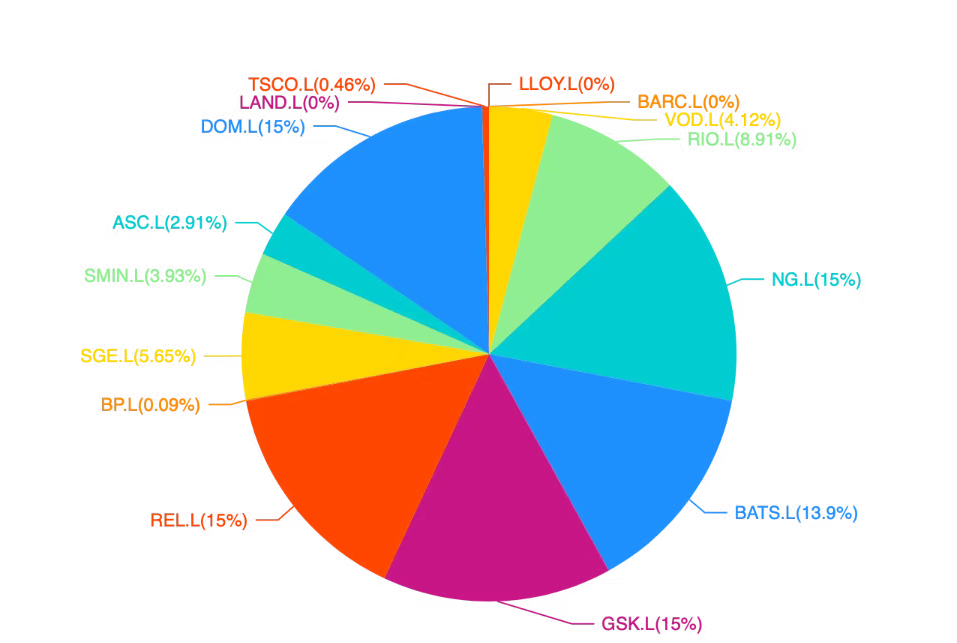
\includegraphics[width=15cm]{./Figures/optimal.png}
    \caption{The Optimal Portfolio Combination}
    \label{optimal}
\end{figure}
\end{center}

\hspace*{\fill}\\
Under the model constraint of buying each stock no more than 15\%, our optimal plan of the portfolio invest mostly in 5 sectors: Communication Services, Consumer Defensive, Consumer Cyclical, Utilities and Healthcare. This ensures that we spread out the risk of the investment by investing in the sectors that are less correlated to each other.
\\\hspace*{\fill}\\
We do not invest in the sector "Financial Service", since by computing the average stock return rate, the two stocks we chose in this sector show that their average returns are negative: the Lloyds Bank has a negative return rate of $-62.9\%$, while the Barclays is of $-22.8\%$.
\\\hspace*{\fill}\\

Based on our model, we see that in this situation we will receive $1.2\%$ of stock returns with the risk $0.138781605\%$. Subsequently we shall show our target asset allocation in this situation. The following table illustrates our selection on the portfolio combinations, consisting of 15 stocks.

\begin{center}
\begin{tabular}{ |p{4cm}|p{1.5cm}|p{2.5cm}|p{2.5cm}|  }
\hline
%\multicolumn{4}{|c|}{The Information of the Portfolio Combinations} \\
%\hline
Company Name& Stock index & Sector type & Asset Allocation\\
\hline
Lloyds Banking Group plc & LLOY.L & Financial Services & $0\% (0 \textit{\pounds} )$ \\
\hline
Barclays PLC & BARC.L & Financial Services & $0\% (0 \textit{\pounds} )$\\
\hline
Vodafone Group Public Limited Company & VOD.L & Communication Services & $4.121\% (12363 \textit{\pounds})$ \\
\hline
RELX PLC & REL.L & Communication Services & $15\% (45000 \textit{\pounds})$ \\
\hline
Tesco PLC & TSCO.L & Consumer Defensive & $0.463\% (1389 \textit{\pounds})$ \\
\hline
British American Tobacco p.l.c. & BATS.L & Consumer Defensive & $13.927\% (41781 \textit{\pounds})$ \\
\hline
ASOS Plc & ASC.L & Consumer Cyclical & $2.905\% (8715 \textit{\pounds})$ \\
\hline
Domino's Pizza Group plc & DOM.L & Consumer Cyclical & $15\% (45000 \textit{\pounds})$ \\
\hline
Rio Tinto Group & RIO.L & Basic Material & $8.906\% (26718 \textit{\pounds})$ \\
\hline
National Grid plc & NG.L & Utilities & $15\% (45000 \textit{\pounds})$ \\
\hline
GlaxoSmithKline plc & GSK.L & Healthcare & $15\% (45000 \textit{\pounds})$\\
\hline
BP p.l.c. & BP.L & Energy & $0.0885\% (265.5 \textit{\pounds})$ \\
\hline
The Sage Group plc & SGE.L & Technology & $5.655\% (16995 \textit{\pounds})$ \\
\hline
Smiths Group plc & SMIN.L & Industrials & $3.934\% (11802 \textit{\pounds})$ \\
\hline
Land Securities Group plc & LAND.L & Real Estate & $0\% (0 \textit{\pounds} )$ \\
\hline
Total & & & $100\% (300000 \textit{\pounds} )$\\
\hline
\end{tabular}
\end{center}

\newpage